\documentclass[12pt]{article}
\usepackage{amsfonts,amssymb}
\usepackage{amsmath}
\usepackage{amsthm}
\usepackage{hyperref}
\usepackage{graphicx}
\usepackage{listings}
%\documentstyle[12pt,amsfonts]{article}
%\documentstyle{article}

\setlength{\topmargin}{-.5in}
\setlength{\oddsidemargin}{0 in}
\setlength{\evensidemargin}{0 in}
\setlength{\textwidth}{6.5truein}
\setlength{\textheight}{8.5truein}
%
%\input ../adgeomcs/lamacb.tex
%\input ../mac.tex
%\input ../mathmac.tex
%
\input xy
\xyoption{all}
\def\fseq#1#2{(#1_{#2})_{#2\geq 1}}
\def\fsseq#1#2#3{(#1_{#3(#2)})_{#2\geq 1}}
\def\qleq{\sqsubseteq}
\newtheorem{theorem}{Theorem}
%cis51109hw1

%
\begin{document}
\begin{center}
\fbox{{\Large\bf Tricky Combinatorics}}\\
\vspace{1cm}
\end{center}


\medskip\noindent

{\bf Notes.}

Main concepts

\begin{itemize}
\item Arrangements when some objects are alike
\item Counting integer solutions
\end{itemize}
\vspace{0.5cm}\noindent

\section*{Arrangements of non-distinct}

\paragraph*{•}
Example - How many ways can the letters of the word WILL be rearranged?

If this question was posed instead as in how many ways can the letters of the word WILD be rearranged, then it becomes quite simple. After all, in that case, it is the arrangement of 4 distinct objects and by this stage you know the answer to that is just 4!

So let us just consider one of the Ls to be in lowercase. Then again, the answer will be 4! But now we are overcounting. We are overcounting because it doesn't matter if the L is in uppercase or lowercase, that was just a step we made in order to make our counting easier.

something like lWIL is the same as LWIl when we do the counting. This is same as as 2 of these map to 1 word.

So if we use the k to 1 concept, all we need to do is $\frac{4!}{2}$.

What is generalization? If instead of 2 Ls we had a word with 3, then think of the 3 Ls as being interchangeable in any word. So any of the 3! arrangements would map to the same word!

\begin{theorem}
If there are $k$ objects in total. $k_1$ of them are of type 1, $k_2$ are of type 2 and so on until $k_n$ are of type n, then the total number of possible arrangements of these objects in a straight line are 

\begin{align*}
\frac{k!}{k_1!k_2!\cdots k_n!}
\end{align*}

\end{theorem}

\textbf{Quick example}

In how many ways can the letters of the word PHILIPPINES be rearranged?

There are PHI LIP PIN ES (Spaces just added to make counting easy) 11 characters in total. 3 Ps and 3 Is. 

So using the previous result $\frac{11!}{3!3!}$

\section*{Counting integer solutions to certain types of equations}

A very popular and powerful combinatorics problem is to count the number of non-negative integer solutions to certain types of equations.

For instance, how many non-negative integer solutions can be found for the following equation

$x_1 + x_2 + x_3 = 8$

We want each of the $x_i$s to take on a non-negative value. 

At least initially, this question looks quite different from anything related to the arrangement of objects. But there is a small trick that reduces it to one of the problems seen before.

Consider the following mapping between solutions of the equations and arrangements of identical balls.

Given a solution of the equation like 5, 2, 1 ($x_1 = 5$, $x_2 = 2$ and $x_3 = 1$ ) we can map it to

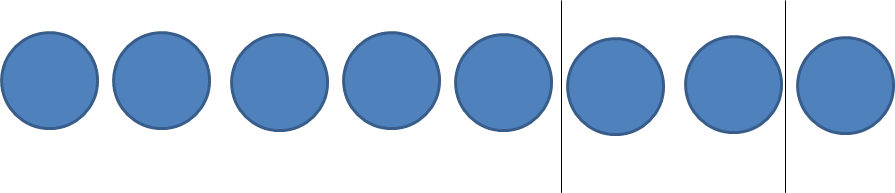
\includegraphics[scale=0.5]{./img/Separators.png}

That is an arrangement of identical balls with 2 separators placed in there to distinguish between which set corresponds to $x_1$, which to $x_2$ and the rest correspond to $x_3$.

So our mapping is defined now between the set of non-negative solutions to the equation and the set of arrangements of 8 identical balls and 2 identical separators (while the separators can be placed at different locations, they look exactly the same).

Is this mapping a bijection? 

Given a solution to the equation, we have demonstrated how to construct an arrangement - put down as many balls as the value of $x_1$, then put down a separator. Then put down as many balls as the value of $x_2$. Then put down another separator. Then put down the remaining balls.

Similarly given any arrangement of balls and separators, to get the value of $x_1$, count the number of balls to the left of the first separator. That is $x_1$. Then count the number of balls between the first two separators. That is the value of $x_2$. Finally, count the number of balls to the right of the last separator. That is the value of $x_3$.

Since we have demonstrated how to go from one set to the other in a unique manner (yes this is a hand wavy proof, but having not done mathematical proof yet, we are ok with this), we have a bijection.

So how does one count the number of arrangments of identical balls and separators?

There are 8 balls and 2 separators. That is 10 objects, 8 of 1 kind, 2 of another kind.

$\frac{10!}{8!2!}$

You could also think of it as 10 blank spots to be filled. We have to choose 2 spots to place the separators. That is $\binom{10}{2}$.

\subsection*{Counting multisets}
Typically one thinks of sets as collections of distinct items. However, sets can also be defined in a way that allows them to have multiple instances of the same kind of item. Such sets are called multisets. Multiset is another way of saying a set that repetitions  are allowed.

Given a set $\{1,2,3,4\}$, how many multisets can be formed from it?

The absurdity of the question should hopefully strike you readily. If you are allowed to repeat elements then surely $\{1,1,1\}$ is a multiset. So too $\{1,1,2,3,4,4\}$. There are infinitely many.

But what if we add a constraint on the number of elements. How many $4$ element multisets are there?

This again might initially seem to be unrelated to other problems but what if we did the following. Let $x_1$ represent the number of copies of $1$ in our multiset. Let $x_2$ represent the number of copies of $2$ and so on.

Then we want $x_1 + x_2 + x_3 + x_4 = 4$. And we know how to solve those now! 4 balls, 3 separators. That means $\frac{7!}{4!3!}$.

\section*{Examples dealing with constraints}
This problem shows up in many different forms. I will just refer to it as the girls and boys counting problem. Suppose you have 5 girls and 3 boys. You want to arrange them (in a line) in such a way that you do not have 2 boys standing next to each other. 

The classic way of solving this problem is to first arrange the girls - 5! ways.

Now think of any girl arrangement as G G G G G, that is with these gaps in between them.

Where do the boys go? In the gaps! How many gaps are there? 6 gaps (remember the gaps at the start and end of the line). 

The boys choose the gaps in $\binom{6}{3}$ and then can be rearranged in 3! ways. Alternatively, we can do it directly by saying in how many ways can a set of 3 (boys) be mapped to a set of 6 (gaps).

Putting it all together we get $5! \cdot 6\cdot 5\cdot 4$.  


\end{document}



